\section{Example}

\begin{frame}<1-4>{Frame with 4 States}%
    \begin{Def}
      State one 
      \uncover<2->{
        \begin{align}
          T(s):=C'(s) & & \kappa(s):=|T'(s)| 
        \end{align}  
        State two
      }%
      \uncover<3>{State three}%
      \uncover<4>{State four}
  
      \begin{columns}
        \begin{column}{0.3\textwidth}
          \begin{align}
            \uncover<3->{N(s):=\frac{T'(s)}{|T'(s)|} } \\
            \\
            \uncover<4->{B(s):= T(s) \times N(s)}
          \end{align}
        \end{column}
  
        \begin{column}{0.6\textwidth}
          \begin{tikzpicture}
            \only<2>{\node[inner sep=0pt] (ribbon) at (0,0)
                {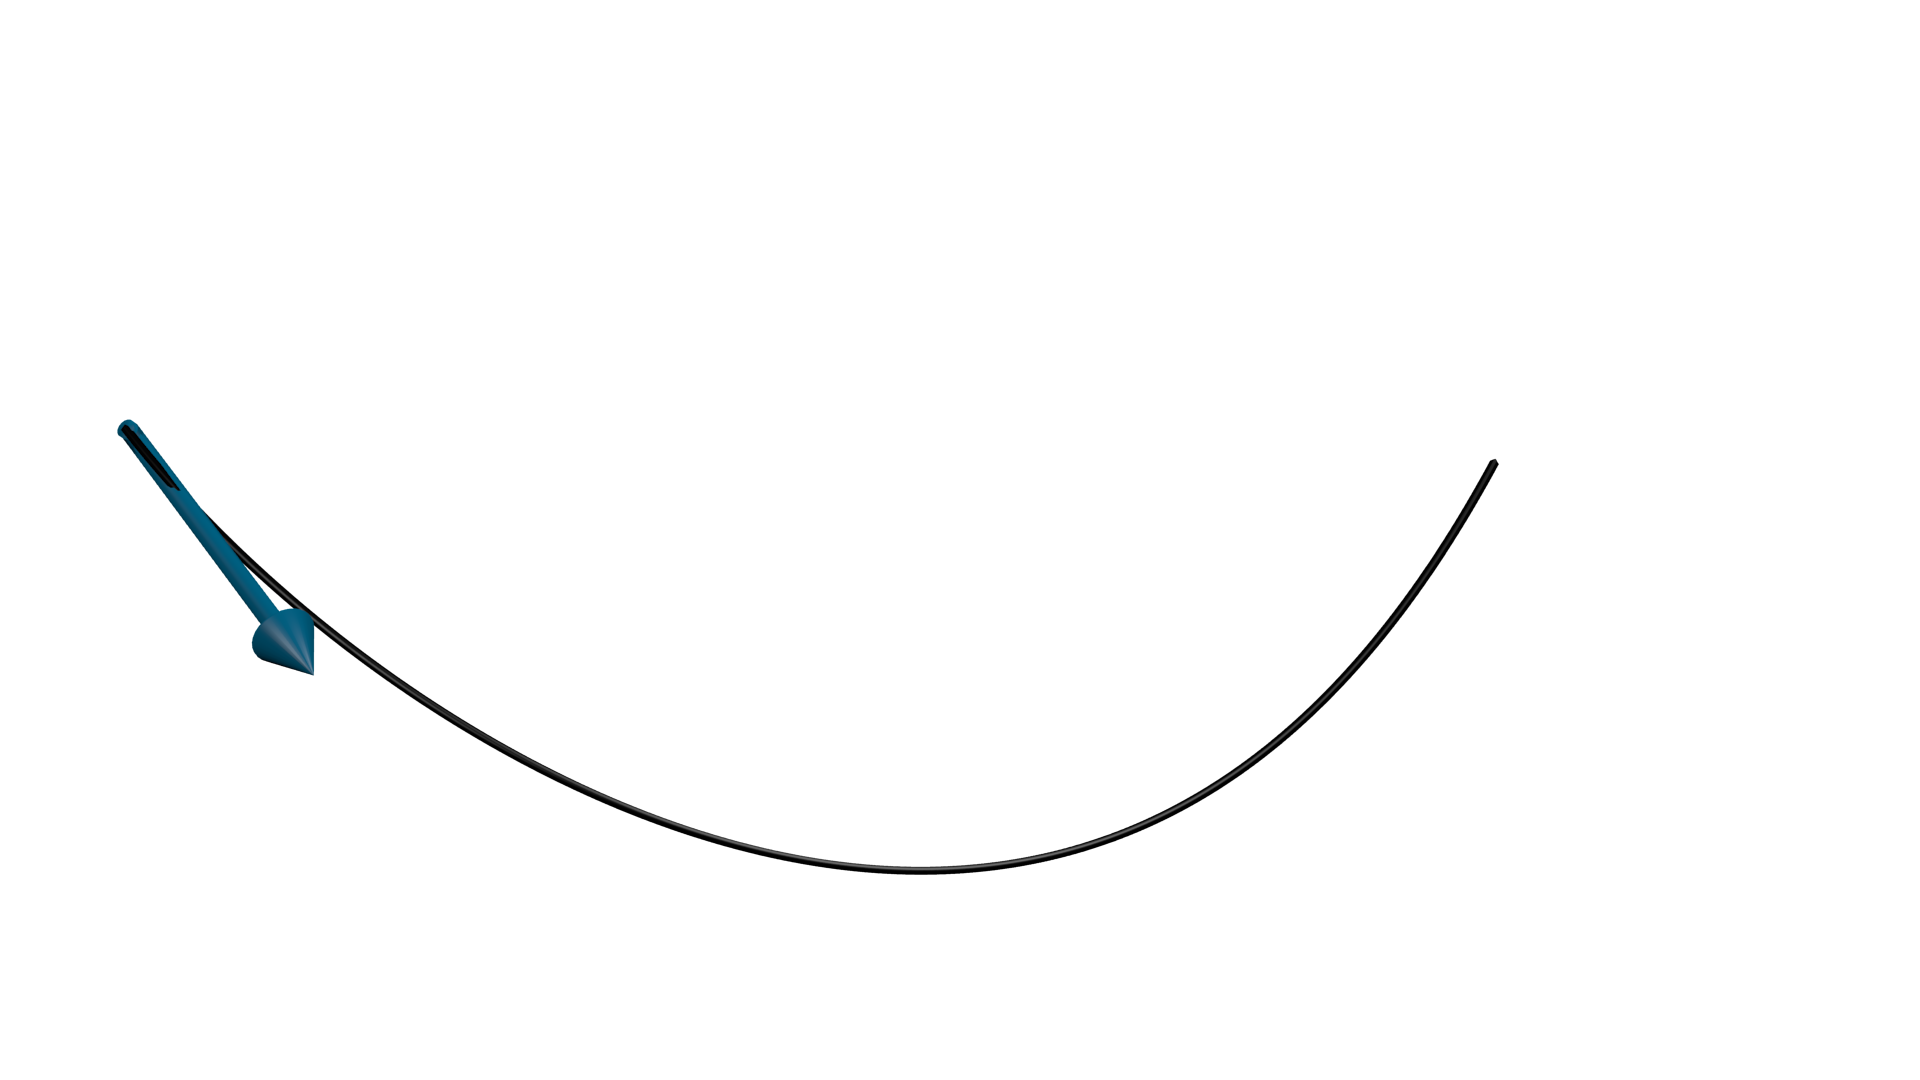
\includegraphics[width=7cm]{../graphics/Frenet_Tan.png}};
            }
            \only<3>{
            \node[inner sep=0pt] (ribbon) at (0,0)
                {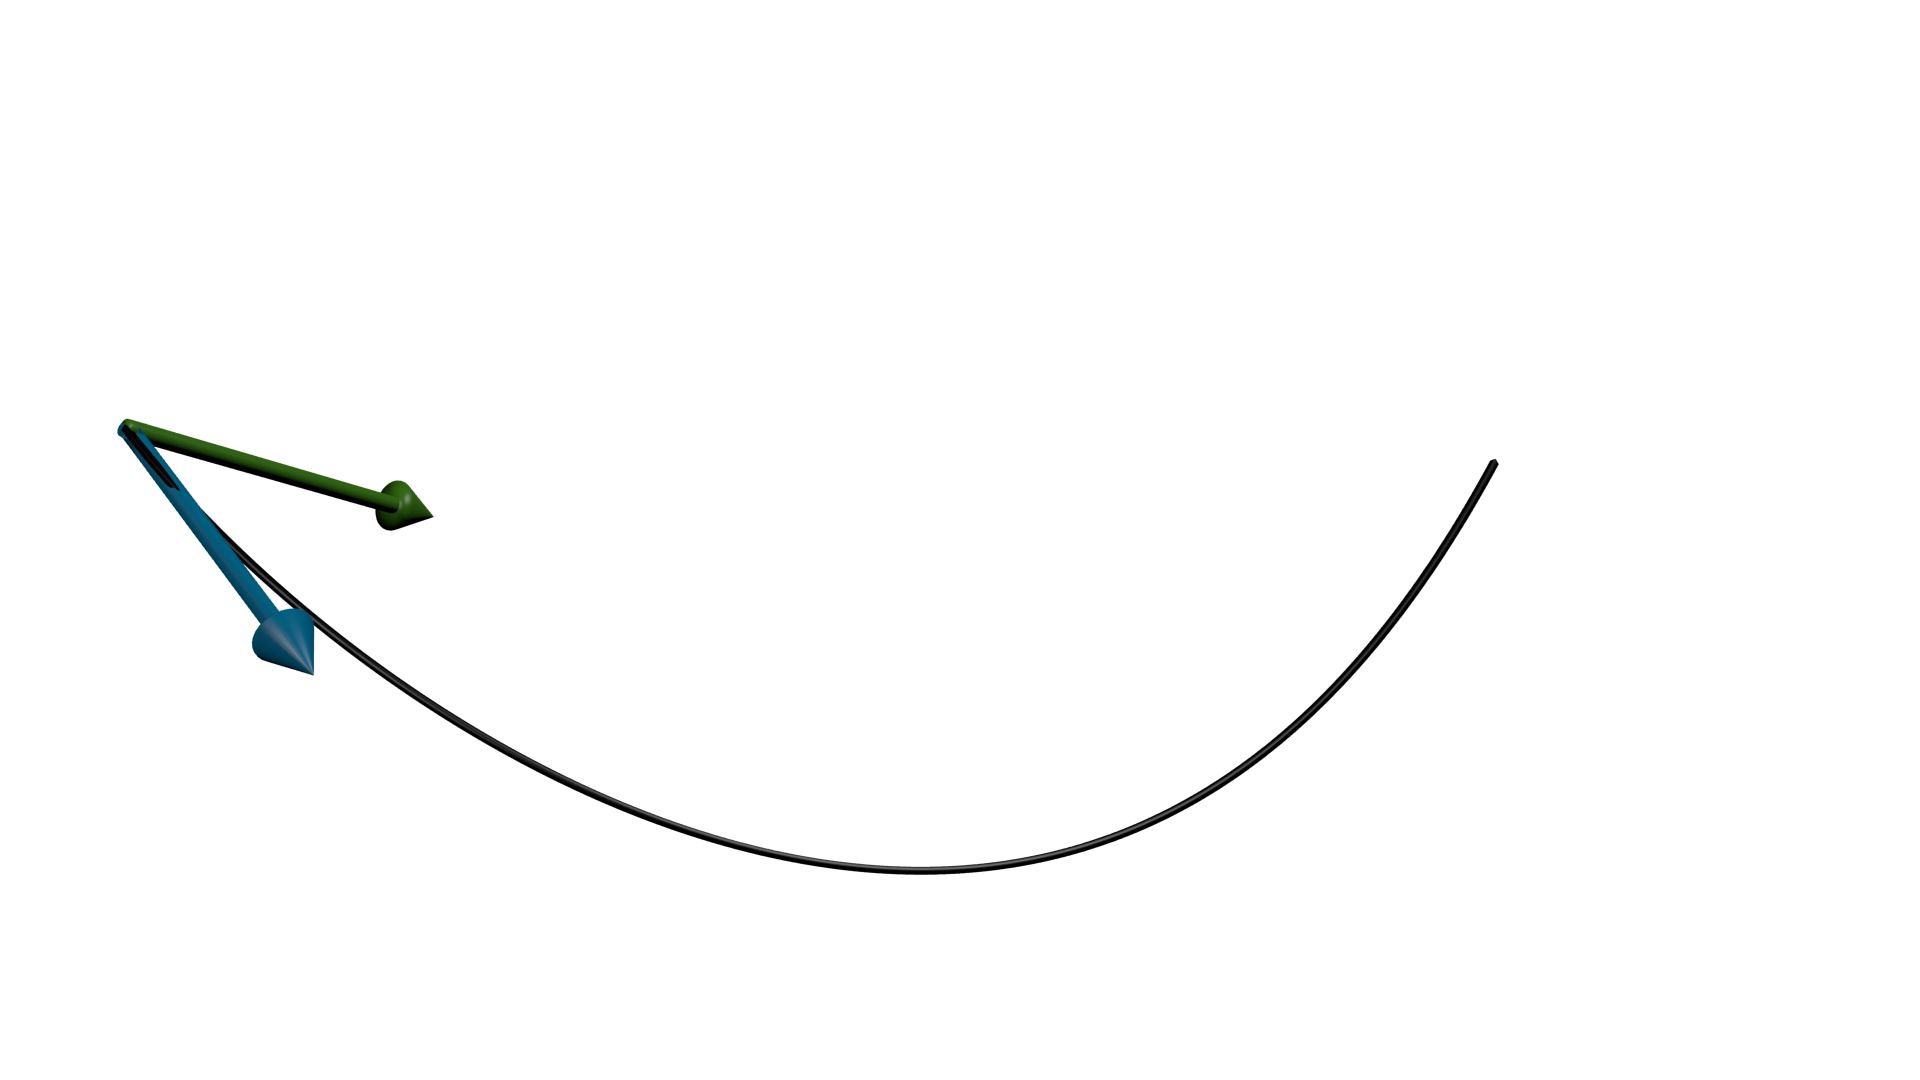
\includegraphics[width=7cm]{../graphics/Frenet_Tan_Nor.png}};
            }
            \uncover<4->{
            \node[inner sep=0pt] (ribbon) at (0,0)
                {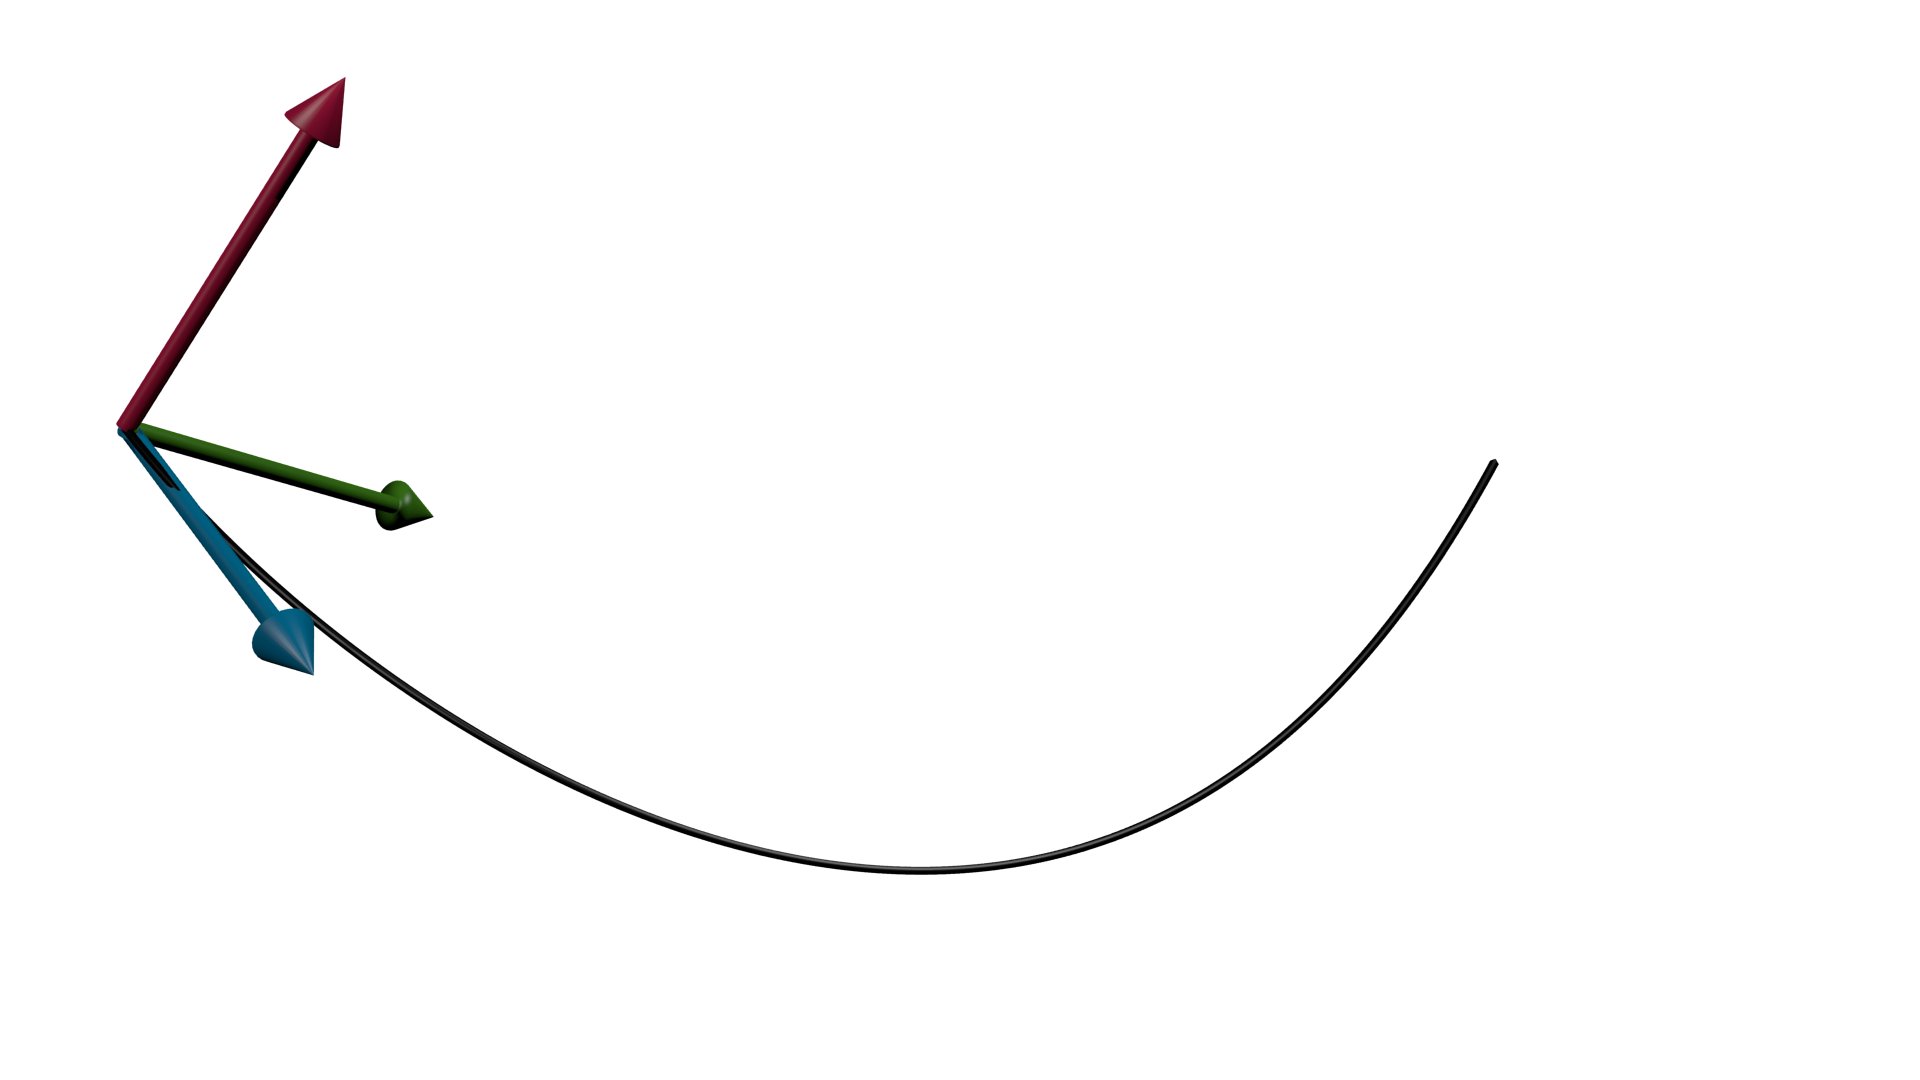
\includegraphics[width=7cm]{../graphics/Frenet_Tan_Nor_Bin.png}};
            }
            \uncover<2->{\node[inner sep=0pt, anchor=east] (C) at ($(ribbon.east) + (-1.4,0.6)$) {$C$};
            \node[inner sep=0pt, anchor= west] (T) at ($(ribbon.west) + (1.2,-0.7) $) {\textcolor{rwthblue}{$T$}};
            }
            \uncover<3->{
            \node[inner sep=0pt, anchor=south] (N) at ($(ribbon.north) + (-1.7,-2)$) {\textcolor{rwthgreen}{$N$}};
            }
            \uncover<4->{
            \node[inner sep=0pt, anchor= south] (B) at ($(ribbon.north) + (-2,-0.3) $) {\textcolor{rwthmagenta}{$B$}};
            }
        \end{tikzpicture}
        \end{column}
      \end{columns} 
      
    \end{Def}
  
    \note{
      %\trickdown %wird manchmal benötigt um den State-Zähler in Frame und Notes zu synchronisieren. Habe noch nicht rausgefunden was der Grund dafür ist.
      \begin{enumerate}
        \item<1-> Bogenl-Param => $|T|=1$
        \item<2-|alert@2> Wir betrachten jetzt Kurven mit pos Krümmung
      \end{enumerate}
    }
  \end{frame}
